% http://www.texample.net/tikz/examples/coin-flipping/
\newcommand{\figwidth}{\textwidth}
\newcommand{\leveldistance}{8pt}
\newcommand{\tpdistance}{16pt}
\newcommand{\tphalfheight}{6pt}
\newcommand{\tpdescwidth}{32pt}

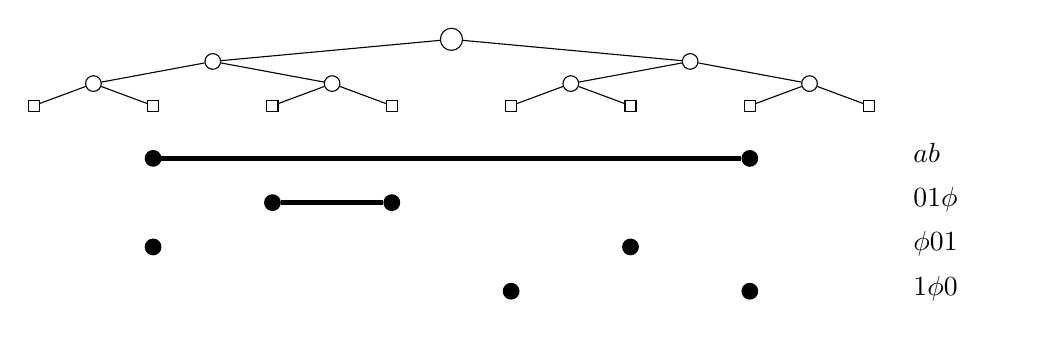
\begin{tikzpicture}[
    %scale = 1,
    %transform shape,
    %thick,
    %grow = down,  % alignment of characters
    level 1/.style = {sibling distance=\figwidth / 2},
    level 2/.style = {sibling distance=\figwidth / 4},
    level 3/.style = {sibling distance=\figwidth / 8},
    level distance = \leveldistance,
    inner/.style = {draw, circle, inner sep=2pt},
    leaf/.style = {inner, rectangle},
    root/.style = {inner, minimum size=8pt},
    point/.style = {draw, circle, inner sep=2pt},
    truepoint/.style = {point, fill = black},
    falsepoint/.style = {point, fill = white},
    trueinterval/.style = {line width = 2pt},
    tpdesc/.style = {text width = \tpdescwidth}
  ]
  \node[root] (eps) {}
   child { node[inner] (0) {}
     child { node[inner] (00) {}
       child { node[leaf] (000) {}}
       child { node[leaf] (001) {}}
     }
     child { node[inner] (01) {}
       child { node[leaf] (010) {}}
       child { node[leaf] (011) {}}
     }
   }
   child {   node[inner] (1) {}
     child { node[inner] (10) {}
       child { node[leaf] (100) {}}
       child { node[leaf] (101) {}}
     }
     child { node[inner] (11) {}
       child { node[leaf] (110) {}}
       child { node[leaf] (111) {}
         child [grow=right, level distance=32pt] {node (A) {} edge from parent[draw=none]}
       }
     }
   };

  \begin{scope}[nodes = {draw = none}]
    \begin{scope}[nodes = {below = \tpdistance}]
      \node [name = a, truepoint] at (001) {};
      \node [name = b, truepoint] at (110) {};
      \draw [trueinterval] (a) -- (b) node {};
    \end{scope}
    \node [tpdesc, below=\tpdistance - \tphalfheight] at (A) {$\interval{a}{b}$};
    \begin{scope}[nodes = {below = \tpdistance * 2}]
      \node [name = 01p010, truepoint] at (010) {};
      \node [name = 01p011, truepoint] at (011) {};
      \draw [trueinterval] (01p010) -- (01p011) node {};
    \end{scope}
    \node [tpdesc, below=\tpdistance * 2 - \tphalfheight] at (A) {$01 \phi$};
    \begin{scope}[nodes = {below = \tpdistance * 3}]
      \node [truepoint] at (001) {};
      \node [truepoint] at (101) {};
    \end{scope}
    \node [tpdesc, below=\tpdistance * 3 - \tphalfheight] at (A) {$\phi 01$};
    \begin{scope}[nodes = {below = \tpdistance * 4}]
      \node [truepoint] at (100) {};
      \node [truepoint] at (110) {};
    \end{scope}
    \node [tpdesc, below=\tpdistance * 4 - \tphalfheight] at (A) {$1 \phi 0$};
  \end{scope}
\end{tikzpicture}